\documentclass[a4paper,12pt,french]{book}
\usepackage[margin=2cm]{geometry}
\usepackage[thinfonts,latinmath]{uglix2}
\usepackage{colortbl}


\setcounter{chapter}{6}
\begin{document}
	\chapter{Algèbres de Boole}
	\begin{center}
		\ \\[-4em]	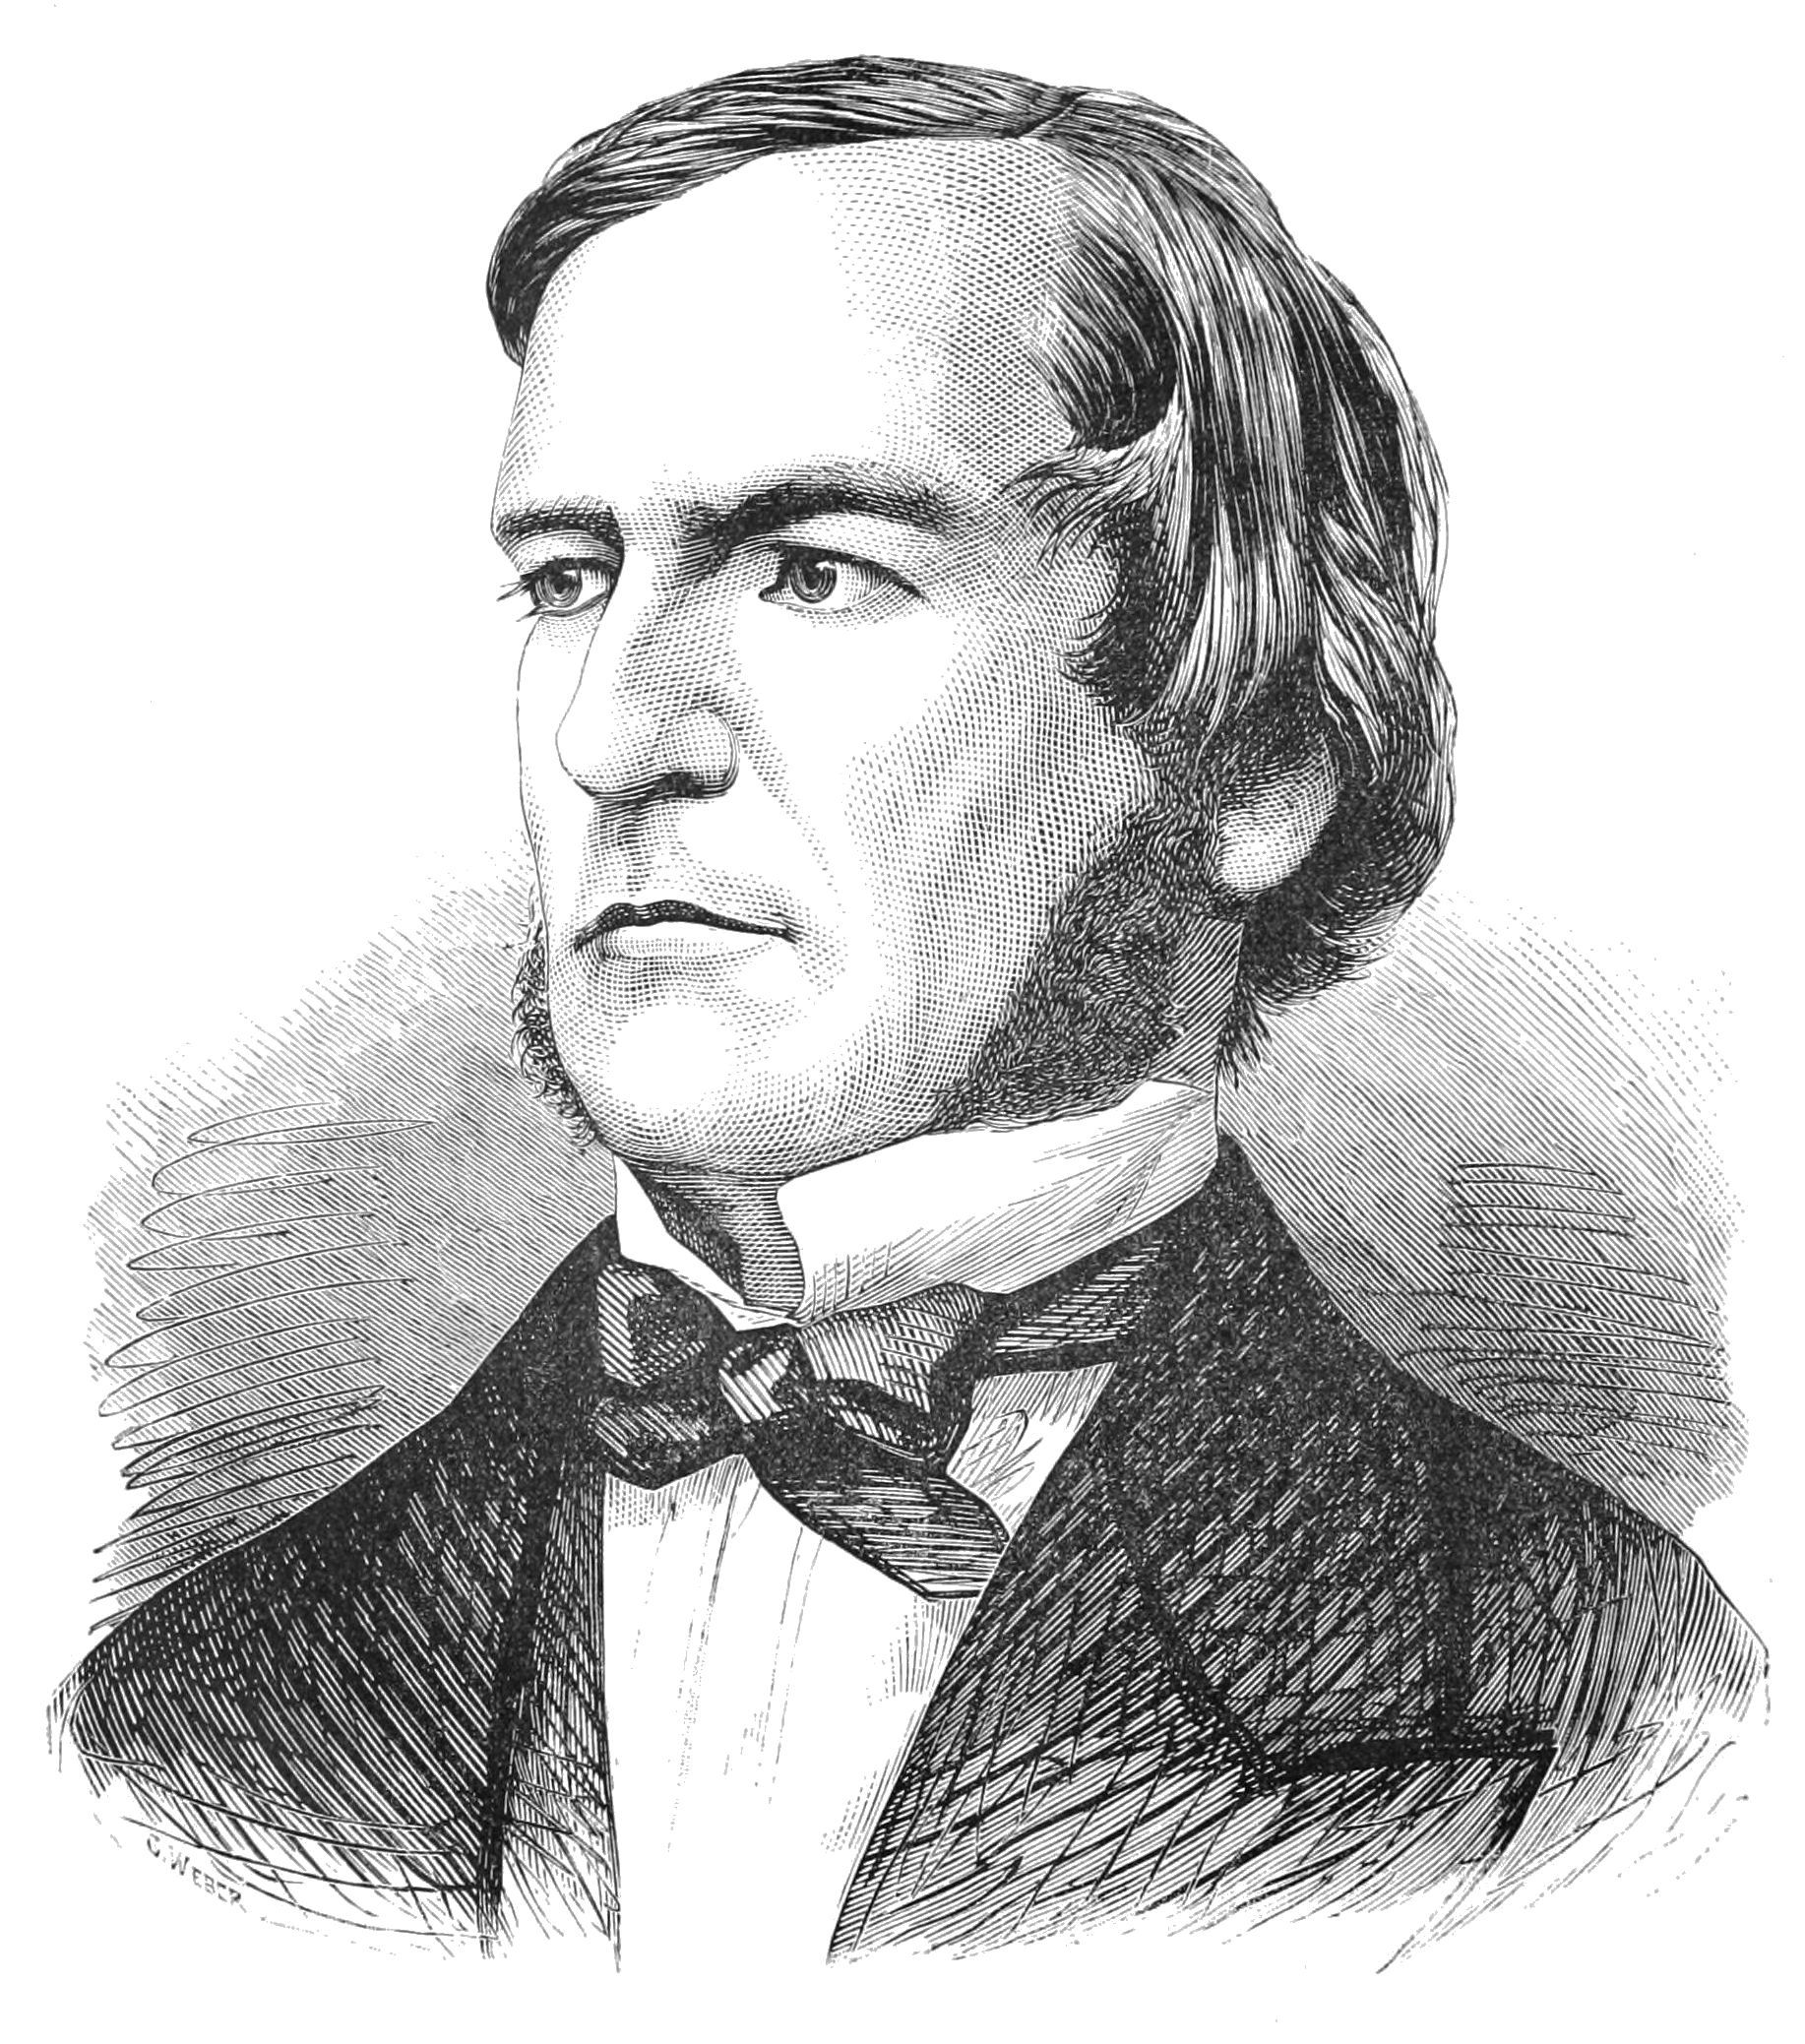
\includegraphics[width=4cm]{boole.jpg}
	\end{center}\ \\[-4em]
	\section{Définition d'une algèbre de Boole}

	\begin{definition}[]
		Une \textit{algèbre de Boole}, c'est un ensemble $E$ muni de :
		\begin{enumerate}[\textbullet]
			\item 	deux lois \textit{binaires} notées + et $\times$;
			\item 	une loi \textit{unaire} qui à $a$ associe $\barmin{a}$;
			\item 	deux éléments particuliers notés 0 et 1;
		\end{enumerate}
		et telle que , pour tous éléments a, b et c de E :
		\begin{enumerate}[\textbullet]
			\item 	Les deux lois binaires sont \textit{commutatives} :
					$a+b=b+a$ et $ab=ba$
			\item 	elles sont aussi associatives :
					$a+(b+c)=(a+b)+c$ et $a(bc)=(ab)c$
			\item 	$\times$ se distribue sur + :
								$a(b+c)=ab+ac$
			\item 	+ se distribue sur $\times$ :
					$\boxed{a+bc=(a+b)(a+c)}$  \\
                    c'est la seule propriété contre-intuitive, on la notera $(*)$
			\item 	0 est neutre pour +: $0+a = a$
			\item 	0 est absorbant pour $\times$ : $0a=0$
			\item 	1 est neutre pour $\times$ : $1a=a$
			\item 	1 est absorbant pour + : $1+a=1$
			\item 	on a $a+\barmin{a}=1$ et $a\barmin{a}=0$
		\end{enumerate}
		\end{definition}



	\begin{exemple}[s]
		\begin{enumerate}[\textbullet]
			\item 	L'ensemble $\{0;1\}$ muni de $\vee$, $\wedge$ et $\neg$ est la plus simple des algèbres de Boole.
			\item 	Si on pose que deux propositions sont égales quand elles sont équivalentes, alors l'ensemble des propositions muni de $\vee$, $\wedge$ et $\neg$ est une algèbre de Boole,
					0 étant la proposition fausse et 1 la proposition vraie.
			\item 	Comme on le verra au prochain chapitre, lorsqu'on se donne un ensemble $E$ et que l'on considère $\mathcal{P}(E)$, l'ensemble de ses parties, muni des opérations $\cap$ (intersection, joue le rôle de $\times$ ) et $\cup$ (union, joue le rôle de +), alors $P(E)$ est une algèbre de Boole, 0 étant l'\textit{ensemble vide} et 1 étant E lui-même.
		\end{enumerate}
	\end{exemple}

	\begin{exercice}[]
		Montrer que :
		\begin{enumerate}[\bfseries a.]
			\item 	$(a+b)(\barmin{a}+c)(\barmin{b}+\barmin{c})=a\barmin{b}c+\barmin{a}b\barmin{c}$
			\item 	$\barmin{a}\barmin{b}\barmin{c}\barmin{d}+a\barmin{b}\barmin{c}\barmin{d}+	\barmin{a}b\barmin{c}\barmin{d}+ab\barmin{c}\barmin{d}=\barmin{b}\barmin{c}$
			\item 	$ab+\barmin{a}\barmin{b}+ \barmin{a}b=\barmin{a}+b$

		\end{enumerate}
	\end{exercice}

	\begin{propriete}[s]
		\begin{enumerate}[\textbullet]
			\item 			Dans une algèbre de Boole, pas besoin de multiplication par un entier car pour tout élément $a$ :
			$$a+a = a$$
			Donc $2a = a$ et par suite pour tout entier naturel non nul $n$ : $na=a$.
			\item Pas besoin de puissances non plus  car pour tout élément $a$ :
			$$aa = a$$
			Donc $a^2 = a$ et par suite pour tout entier naturel non nul $n$ : $a^n=a$.\\

		\end{enumerate}
	\end{propriete}

	\textbf{Preuve :}\\

	Soit $a$ un élément de E:
	\begin{multicols}{2}
	\begin{enumerate}[\textbullet]
		\item 	\begin{tabbing}
			$a$ \= 	$=a+0$\\
				\>	$=a+a\barmin{a}\qquad$ et on utilise $(*)$\\
				\>	$=(a+a)(a+\barmin{a})$\\
				\>	$=(a+a)1$\\
				\>	$=a+a$
		\end{tabbing}
		\item 	\begin{tabbing}
			$a$ \= $=a\times 1$\\
				\> $=a(a+\barmin{a})$\\
				\> $=aa+a\barmin{a}$\\
				\> $=aa+0$\\
				\> $=aa$
		\end{tabbing}
	\end{enumerate}
	\end{multicols}
	\begin{propriete}
		Si 2 éléments $x$ et $y$ de E sont tels que $xy=0$ et $x+y=1$, alors $x=\barmin{y}$.
	\end{propriete}
\textbf{Preuve :}
\begin{tabbing}
	$x+y=1\quad$	\=	$\Rightarrow\quad (x+y)\barmin{y}=\barmin{y}$\\
					\>	$\Rightarrow\quad x\barmin{y}+y\barmin{y}=\barmin{y}$\\
					\>	$\Rightarrow\quad x\barmin{y}+0=\barmin{y}$\\
					\>	$\Rightarrow\quad x\barmin{y}+xy=\barmin{y}$\\
					\>	$\Rightarrow\quad x(\barmin{y}+y)=\barmin{y}$\\
					\>	$\Rightarrow\quad x\times 1=\barmin{y}$\\
					\>	$\Rightarrow\quad x=\barmin{y}$
\end{tabbing}

	\begin{propriete}[ : lois de De Morgan]
		Quels que soient les éléments de $x$ et $y$ de E on a $$\barmin{x\times y}=\barmin{x}+\barmin{y}  \qquad\textrm{et}\qquad \barmin{x+y}=\barmin{x}\times\barmin{y}$$
	\end{propriete}

\textbf{Preuve de la première égalité}.\\
 Si on pose $A=xy$ et $B=\barmin{x}+\barmin{y}$, alors on doit montrer que $\barmin{A}=B$.\\
On utilise la propriété précédente et on montre donc que $A+B = 1$ et que $AB=0$ :
\begin{multicols}{2}

	\begin{tabbing}
		$B+A$ 	\=	$=\barmin{x}+\barmin{y}+xy$ et on utilise $(*)$\\
				\>	$=(\barmin{x}+\barmin{y}+x)(\barmin{x}+\barmin{y}+y)$\\
				\>  $=(1+\barmin{y})(1+\barmin{x})$\\
				\>  $=1\times 1$\\
				\> 	$=1$
	\end{tabbing}

	\begin{tabbing}
		$AB$ \=  $=(\barmin{x}+\barmin{y})xy$\\
		\>  $=\barmin{x}xy+\barmin{y}xy$\\
		\> 	$=0y+0x$\\
		\> 	$=0+0$\\
		\> 	$=0$
	\end{tabbing}
\end{multicols}
\begin{exercice}[]
	Montrer la deuxième loi en faisant la même chose.
\end{exercice}



\section{Diagrammes de Karnaugh}

Cette méthode a été développée par Maurice Karnaugh en 1953. Elle fait appel à des tableaux qui représentent des expressions booléennes.\\
On colorie les cases qui correspondent aux différents termes de l'expression. À la fin on peut reconnaître et lire une expression simplifiée.

\begin{propriete}[]
	Un produit correspond à une \textit{intersection}, une somme à une \textit{union}.
\end{propriete}

\subsection*{Avec 2 variables}

Le diagramme est un carré dont les quatre cases correspondent aux quatre produits $ab$, $a\barmin{b}$, $\barmin{a}b$, $\barmin{a}\barmin{b}$.

\begin{center}
	\begin{tabular}{|c|c|}
		\hline
		$ab$ &  $a\barmin{b}$\\
		\hline
		$\barmin{a}b$ & $\barmin{a}\barmin{b}$\\
		\hline
	\end{tabular}
\end{center}
Ci dessous on représente a, b, $\barmin{a}$, $\barmin{b}$ et une dernière expression.
\begin{center}
	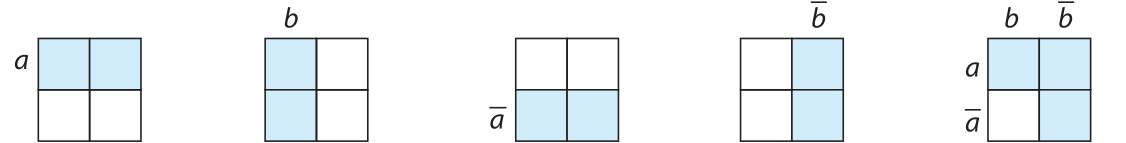
\includegraphics[width=15cm]{karnaugh1.png}
\end{center}

Cette dernière peut se lire $a+\barmin{b}$ ou bien $ab+a\barmin{b}+\barmin{a}\barmin{b}$.

\begin{exercice}[]
	Propose une troisième interprétation du dernier diagramme.
\end{exercice}

\subsection*{Avec 3 variables}

Le diagramme est un rectangle dont les huit cases correspondent aux produits suivants.

\begin{center}
	\begin{tabular}{|c|c|c|c|}

		\hline
		$abc$ & $ab\barmin{c}$ & $a\barmin{b}\barmin{c}$ &  $a\barmin{b}c$\\
		\hline
		$\barmin{a}bc$ & $\barmin{a}b\barmin{c}$ & $\barmin{a}\barmin{b}\barmin{c}$ &  $\barmin{a}\barmin{b}c$\\
				\hline
	\end{tabular}
\end{center}
\begin{center}
	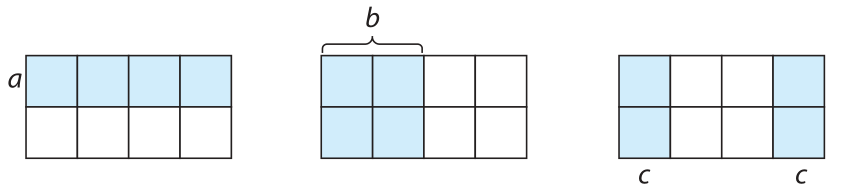
\includegraphics[width=15cm]{karnaugh2.png}\\

	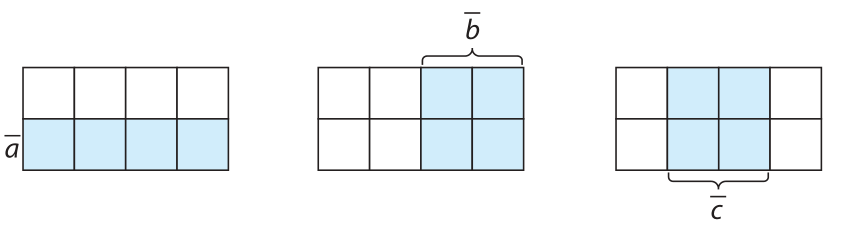
\includegraphics[width=15cm]{karnaugh3.png}
\end{center}

\begin{exercice}[]
	Faire les tables de Karnaugh des expressions $ab$, $a\barmin{b}$, $ac$, $a\barmin{c}$,  $\barmin{a}b$, $\barmin{a}\barmin{b}$, $\barmin{a}c$, $\barmin{a}\barmin{c}$, $bc$, $\barmin{b}c$, $b\barmin{c}$, $\barmin{b}\barmin{c}$.
\end{exercice}


\end{document}